% source
% https://latexdraw.com/plot-vector-field-in-latex-tikz/

\documentclass{standalone}
 
\usepackage{pgfplots}
\pgfplotsset{compat = newest}
\pgfplotsset{ticks=none}
\usepgfplotslibrary{colormaps}
 
\begin{document}
 
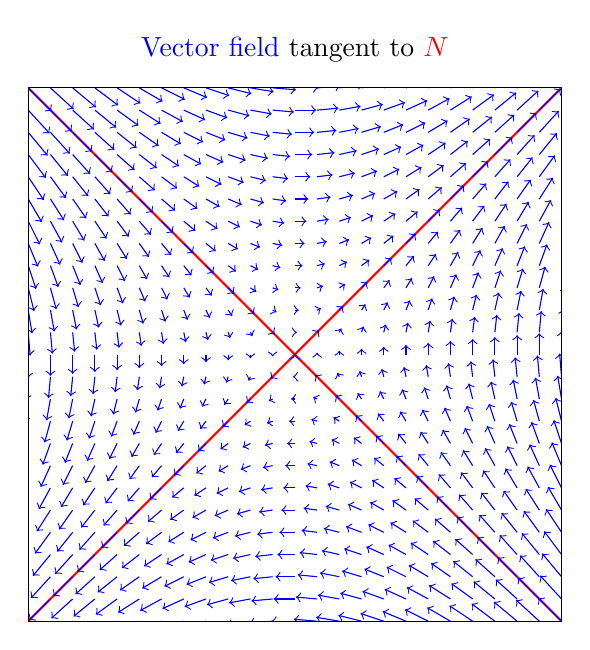
\begin{tikzpicture}
\begin{axis}[
    xmin = -4, xmax = 4,
    ymin = -4, ymax = 4,
    zmin = 0, zmax = 1,
    axis equal image,
    xtick distance = 1,
    ytick distance = 1,
    view = {0}{90},
    scale = 1.25,
    title = { {\color{blue}Vector field} tangent to {\color{red}$N$}},
    height=7cm,
%    axis lines= none,
%    xlabel = {$x$},
%    ylabel = {$y$},
%    colormap/cool,
%    colorbar,
%    colorbar style = {
%        ylabel = {Vector Length}
%    }
]


\addplot[mark=none, red, thick] coordinates {(-4,4) (4,-4)};
\addplot[mark=none, red,thick] coordinates {(-4,-4) (4,4)};
 
\addplot3[
    point meta = {sqrt(x^2+y^2)},
    quiver = {
            u = {sin(y)},
            v = {sin(x)},
            scale arrows = 5,
    },
    quiver/colored = {blue},
    ->,
    domain = -4:4,
    domain y = -4:4,
] {0};


\end{axis}
 
 
\end{tikzpicture}
 
\end{document}
